\section{Performance Analysis of State-of-the-Art ABR Algorithms over QUIC}
\label{chap04:sec:qui-dash}
In this section, we evaluate and compare the performance of various ABR
techniques over \ac{TCP} and \ac{QUIC}. We develop a testbed setup with the help of a standard DASH player from the \ac{DASH} Industry Forum, where we integrate the \ac{DASH} player with \ac{QUIC} and use emulated network environment based on a large pool of pre-collected network traffic traces. With a total of $45$ hours of streaming video data, we have computed three \ac{QoE} metrics -- (a) average playback bitrate, (b) total rebuffering duration, and (c) playback smoothness, while streaming over both \ac{TCP} and \ac{QUIC}. The detailed experimental setup follows. 

\subsection{Experimental Setup}
\label{chap03s2:sec:experimentalSetup}
For a fair comparison between the performance of \ac{DASH} over \ac{TCP} and \ac{QUIC},
we use an experimental test network as shown in \fig\ref{fig:chap03s2:expeirmental_setup}. We use a streaming server to keep all the videos encoded at different video bitrates as mentioned later and a web-based DASH player provided by \ac{DASH-IF} to stream the videos at the client side. To emulate realistic traffic behavior over the test setup, we use a benchmark traffic shaper {\tt Mahimahi}~\cite{mahimahi} and have created {\tt Mahimahi} compatible traces from two publicly available datasets -- (i) a broadband trace from FCC~\cite{dataset-fcc} and (ii) the 3G/HSDPA mobile dataset collected in Norway~\cite{dataset-norway}. 
%\RC{The setup is best describe in the \fig{\ref{fig:chap03s2:expeirmental_setup}}. We put the video streaming server in the different system and client and the traffic shaper in another system. These two systems are connected via a gigabit ethernet. {\tt mahimahi} tool adjust the uplink and downlink bandwidth by allowing or holding packet based on trace which is provided as input. The trace file is contains information when to release a packet in milliseconds scale. It works on IP layer and any transport layer protocol can be used without any modification.} 
\RC{The setup is best described in \fig{\ref{fig:chap03s2:expeirmental_setup}}. We put the video streaming server in the different system and client and the traffic shaper in another system. These two systems are connected via gigabit ethernet. The {\tt mahimahi} tool adjusts the uplink and downlink bandwidth by allowing or holding IP packets based on the trace provided as input. The trace file contains information on when to release a packet on a milliseconds scale. It works on the IP layer, and any transport layer protocol can be used without any modification.}

\begin{figure}[h]
	\centering
	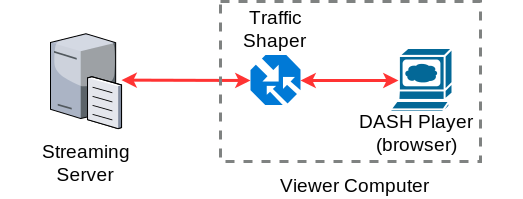
\includegraphics[width=0.8\linewidth]{img/experimental_setup}
	\caption{\label{fig:chap03s2:expeirmental_setup}Experimental setup for video streaming using DASH}
\end{figure}

We run two servers with different end-to-end data transfer protocols, one for \ac{QUIC} and another for \ac{TCP}. For \ac{QUIC} server, we use the {\tt golang} implementation of \ac{QUIC} -- \texttt{GO-QUIC}\footnote{\url{https://github.com/lucas-clemente/quic-go} (\lastaccessedtoday)} (release version 12.0). We have also tested with other \ac{QUIC} implementations like LiteSpeed \ac{QUIC}~\footnote{\url{https://github.com/litespeedtech/lsquic} (\lastaccessedtoday)} and have similar observations as reported in this chapter. We give the results corresponding to the \texttt{GO-QUIC} implementation as it has been used by majority of the existing works in literature. For TCP based server, we use the standard {\tt webfsd}\footnote{https://www.gsp.com/cgi-bin/man.cgi?section=1\&topic=webfsd (\lastaccessedtoday)} web-server (version 1.21). As only the {\tt Google Chrome} and the {\tt Chromium} browsers support the \ac{QUIC} protocol, we use the {\tt Google Chrome} browser of compatible version 68, for our experiments to stream the videos at the client side over the \ac{DASH-IF} streaming player.


In all the experiments, we use off-the-shelf applications and run them in a non-root user mode. The streaming server and the \ac{DASH} players run over systems with 8GB of RAM and Intel(R) Core(TM) i5-4590 CPU @ 3.30GHz processor running Ubuntu 16.04.6 LTS operating system on top of Linux 4.9.78. For \ac{DASH} client, we modify dash.js v2.9.3 to add support for advance \ac{ABR} algorithms like Pensieve and MPC.


\begin{table}[h]
     \caption{\label{table:chap03s2:bitrate}Bitrate and resolution map of DASHified videos.}
	\centering
	\begin{tabular}{|l|c|c|c|c|}
		\hline
		Bitrate(kbps) & 200 & 400 & 600 & 800 \\ \hline
		Resolution & 320x180 & 320x180 & 480x270 & 640x360 \\ \hline \hline
		Bitrate(kbps) & 1000 & 1500 & 2500 & 4000 \\ \hline
		Resolution & 640x360 & 768x432 & 1024x576 & 1280x720 \\ \hline
	\end{tabular}
\end{table}

We use a total of $45$ hours of videos (about $57$ different videos) which have been dashified (encoded in different bitrates as shown in \tbl\ref{table:chap03s2:bitrate}) using the {\tt ffmpeg} tool in eight different video quality levels and two different audio quality levels. We play every video for all the \ac{ABR} algorithms and protocol combinations, resulting $\approx 19$ days of video playback time. We maintain the similar playback environment for DASH/QUIC and DASH/TCP for each of the video and the \ac{ABR} combinations. 
We have compared the performance across five different \ac{ABR} mechanisms, namely, BOLA (B)~\cite{Spiteri2016}, the standard buffer-based quality adaptation of \ac{DASH-IF} (BB), the two variants of MPC driven approaches~\cite{yin2015control} -- MPC-Fast (MF) and MPC-Robust (MR) and the deep learning driven quality adaptation algorithm -- Pensieve (P)~\cite{mao2017neural}. To measure the overall \ac{QoE} of the video playback, we have used a combined metric of the average quality level, the rebuffering time and the playback smoothness, as used in~\cite{yin2015control,mao2017neural}.
\begin{equation}
QoE=\sum_{i=1}^{N}q(R_i)-\mu\sum_{i=1}^{N}\delta_i-\sum_{i=1}^{N-1} \bigg\vert q(R_{i+1})-q(R_i)  \bigg\vert
\label{eqn:chap03s2:QoE}
\end{equation}
We modify \eqn\ref{eqn:QoE} as \eqn\ref{eqn:chap03s2:QoE}, which indicates the \ac{QoE} metric to measure the overall \ac{QoE} of a video playback session. Here, $N$ is the total number of chunks for the playback video. $R_i$ and $q(R_i)$ are the representation of the playback bitrate of the chunk $i$ and the quality perceived by a user for that chunk $i$. $\delta_n$ is the rebuffering time for the chunk $i$. $\mu$ is a QoE weight factor \cite{yin2015control}.
We consider a linear representation $q(R_n) = R_n$, similar to~\cite{yin2015control}, indicating that the playback quality increases linearly with the increase of playback bitrate.
